\section{Описание стилевых файлов}
\label{sec:style}

В данном проекте все параметры документа вынесены в стилевые файлы, готовые к распространению\cite{packages}. Они имеют расширение\texttt{*.sty}. При составлении данных файлов были учтены следующие стандарты: стандарт оформления ИРНИТУ СТО 005-2015\cite{sto005}, ГОСТ 7.32---2001\cite{GOST732}.

За основу взят класс extarticle, так как стандартные классы не поддерживают по умолчанию кегль основного текста более 12pt, согласно стандарту основной текст документа должен быть набран кеглем в 14pt. Также был указан формат листа А4. Подключены дополнительные пакеты для работы с кириллицей и русским языком (fontenc, inputenc, babel, pscyr). Основной кодировкой документа является utf-8.

Пакет \texttt{geometry} определяет поля страницы, согласно вышеуказанным стандартам, отступ от края страницы о границы текста должен быть:
\begin{itemize*}
	\item сверху --- 1.5 см;
	\item справа --- 1 см;
	\item снизу --- 2 см;
	\item слева --- 3 см.
\end{itemize*}

Нумерация страниц указана по центру нижнего колонтитула.

Во всем документе, кроме листингов, использовалась стандартное семейство шрифтов Computer Modern. Гарнитура основного текста --- Roman, заголовков --- Bold Non-extended (начертание полужирное, капитель); моноширинная гарнитура Computer Modern Typewriter.

Основной текст имеет выключку по формату\footnote{англ: justified}. Отступ первой строки абзаца --- 1,25см. Переносы запрещены. Интерлиньяж равен кеглю, это значит, что расстояние между базовыми линиями равно 14pt.

Гарнитура формул --- Latin Modern Math, выключка по центру. Нумерация не использовалась.

Для иллюстраций используется верстка вразрез, при этом для каждого изображения выбирается оптимальный размер --- информация, изображенная на рисунке должна быть легко читаема, но не занимать лишнее пространство на странице.

\subsection{Листинги}
\label{sec:listings}

Подключенный стилевой файл позволяет включать листинги двумя способами: встроенный пакет \texttt{listings} и стороннее приложение-конвертер \texttt{Highlight} t(рисунок~\ref{fig:highlight}).

Преимущество первого метода состоит в том, что при его использовании не требуется предварительное преобразование. В данном проекте используется второй способ, поскольку данное приложение позволяет гибко настроить внешний вид листинга, но при этом автоматическое добавление листинга основного скрипта не использовалось, т.~к. дополнительное преобразование усложнило бы процесс разработки.

\begin{figure}[H]
	\centering
	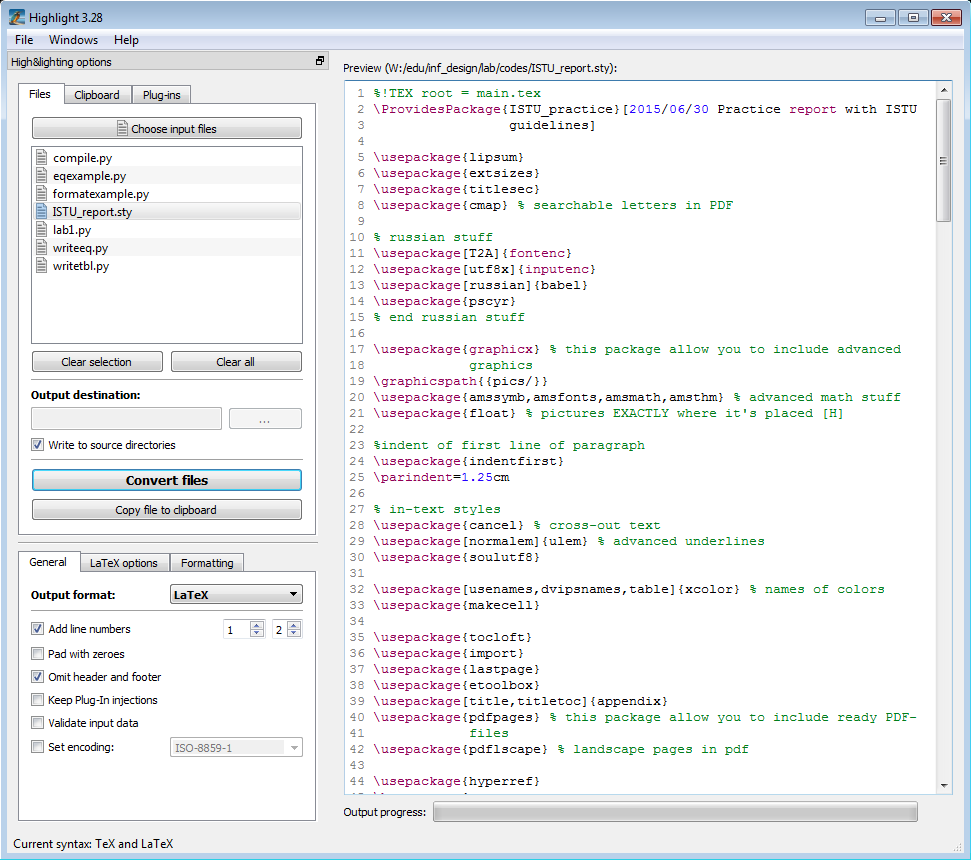
\includegraphics[width=0.8\textwidth]{pics/highlight.png}
	\caption{Приложение highlight}
	\label{fig:highlight}
\end{figure}

Данное приложение преобразовывает исходный текст в язык разметки Latex, автоматически формируя разметку. Также на выходе создается стилевой файл, необходимый для корректного отображения листинга, но данном проекте он уже включен в стилевой файл \texttt{customCodes.sty} (листинг~\ref{lst:customCodes}). Также в результате выполнения экранируются служебные символы.

Гарнитура, используемая в листингах --- свободная, моноширинная Inconsolata. Для сокращения используемого пространства расстояние между базовыми линиями (интерлиньяж) был выбран равный 0.68 от кегля основного текста. Кегль текста был задан как \texttt{\textbackslash footnotesize}, что примерно равно 12pt.

\subsection{Таблицы}
\label{sec:tables}

Для отображения таблиц использовался пакет \texttt{longtables}, который позволяет дублировать заголовки таблиц и в начале каждой новой страницы добавлять текст ``продолжение таблицы...'', как того требуют стандарты.

Для удобства восприятия информации из таблиц, кегль всего текста внутри данного окружения был уменьшен примерно до 12pt, это позволило избежать переносов строк таблицы.

Также в стилевой файл включены такие пакеты, как: \texttt{multicol}, \texttt{multirow}, \texttt{booktabs} для более гибкой настройки таблиц (например, объединение ячеек, определяемый стиль границ), но в данном проекте не использовались.